\documentclass[a4paper,11pt]{article}
\usepackage{graphicx}
\usepackage[margin=1in]{geometry}

\usepackage[table,xcdraw]{xcolor}
\usepackage[utf8]{inputenc}
\usepackage{ulem}
\usepackage{color}
\usepackage{enumerate}
\usepackage{amssymb}
\usepackage{amsmath}
\usepackage {tikz}
\usetikzlibrary{arrows,matrix,positioning,fit}
%\usepackage{bera}
\usepackage{listings}
\usepackage{xcolor}
\usepackage{framed}
\usepackage[hidelinks]{hyperref}
\usepackage{enumitem}
%\setenumerate[2]{label=\roman*.}
\usepackage{blindtext}
\usepackage{fancyhdr}
\pagestyle{fancy}
\usepackage{hhline}
\colorlet{punct}{red!60!black}
\definecolor{background}{HTML}{EEEEEE}
\definecolor{delim}{RGB}{20,105,176}
\colorlet{numb}{magenta!60!black}

\definecolor {processblue}{cmyk}{0.96,0,0,0}

%\setenumerate[1]{label=\textbf{\thesection.\arabic*.}}


\begin{document}
\textbf{Integration of 1-forms on Graphs}

\bigskip

\textbf{Introduction}

\bigskip

Given a connected graph $G=(V,E)$ with $V$ vertices, and $E$ edges and a 
1-form $v: E \rightarrow \mathbb{R}^D$. We're looking for the 0-form 
$x: V \rightarrow \mathbb{R}^D$ minimizing the error:

$$E(x) = \sum_{(i,j) \in E} ||dx_{ij} - v_{ij}||^2$$

where $dx: E \rightarrow \mathbb{R}^D$ is the differential of $x$.

\bigskip

\textbf{Obs. 1}: It is sufficient to consider the case $D=1$, because 
the problem can be reduced to solving $D$ independent 1-D problems on 
the same graph for each coordinate.

\bigskip

\textbf{Obs. 2} (Abuses of notation): We use $V$ to denote both the set 
of vertices and the total number of vertices of the graph. And we denote 
$v$ to the 1-form and $v_i$ is the $i-th$ vertex.

\bigskip

\textbf{Obs. 3}: Vertices and edges can be enumerated in many different 
ways. We will enumerate vertices and edges according to a traversal 
order of a spanning tree. This process determine a consistent 
orientation of the edges: an edge will be oriented from a lower vertex 
to a greater vertex:

$$e_{ij}: v_i \rightarrow v_j \ (for \ i < j)$$

\bigskip

\textbf{Integration process}

\bigskip

The proposed process for integrating $v$ is as follows:

\begin{enumerate}
	\item Construct a spanning tree $T$ for $G$
	\item Choose an order of traversal for $T$ and orient the edges 
	from parent to child
	\item Enumerate the vertices and tree edges according to the order 
	of traversal (See figure~\ref{fig:M1})
	\item We will refer to the remaining graph edges (those which do not 
	belong to the tree) as ``loop-edges". Orient the loop-edges from 
	parent to child.
	\item Construct the oriented incidence matrix $D$: this is an $E \times V$ 
	sparse matrix with one row per graph edge and one column per vertex. 
	For each edge $e_{ij} \ (i < j)$ we set the $i-th$ column entry to $-1$ 
	and the $j-th$ column to $1$ (See figure~\ref{fig:M2}). Rows 
	representing tree-edges are ordered such that the $N-1 \times 
	N-1$ upper-right submatrix is lower triangular.
\end{enumerate}


\begin{figure}
\centering
\begin {tikzpicture}[-latex ,auto ,node distance =3cm ,on grid ,
semithick ,state/.style ={ circle ,top color =white , bottom color = processblue!20 ,
draw,processblue , text=blue , minimum width =1 cm},
edge/.style = {->,> = latex'}]
\node[state] (1) {$1$};
\node[state] (2) [below left=of 1] {$2$};
\node[state] (3) [below  right =of 1] {$3$};
\node[state] (4) [below  left =of 2] {$4$};
\node[state] (5) [below  left =of 3] {$5$};
\node[state] (6) [below  right =of 3] {$6$};
\node[state] (7) [below  left =of 4] {$7$};
\node[state] (8) [below  right =of 4] {$8$};
\node[state] (9) [below  right =of 5] {$9$};
\path (1) edge node {1} (2);
\path (1) edge node {2} (3);
\path (2) edge node {3} (4);
\path (3) edge node {4} (5);
\path (3) edge node {5} (6);
\path (4) edge[red] node {} (5);
\path (4) edge node {6} (7);
\path (4) edge node {7} (8);
\path (5) edge node {8} (9);
\path (8) edge[red] node {} (9);
\end{tikzpicture}

\caption{BFS traversal of a spanning tree. Nodes and edges are 
enumerated according to tree traversal. Edges are oriented from 
parent to child. Red edges correspond to 
$loop-edges$.}
\label{fig:M1}
\end{figure}

\begin{figure}
\centering
%$\begin{pmatrix}
%-1 & 1  & 0  & 0  & 0  & 0 & 0 & 0  & 0 &  \\
%-1 & 0  & 1  & 0  & 0  & 0 & 0 & 0  & 0 &  \\
%0  & -1 & 0  & 1  & 0  & 0 & 0 & 0  & 0 &  \\
%0  & 0  & -1 & 0  & 1  & 0 & 0 & 0  & 0 &  \\
%0  & 0  & -1 & 0  & 0  & 1 & 0 & 0  & 0 &  \\
%0  & 0  & 0  & -1 & 0  & 0 & 1 & 0  & 0 &  \\
%0  & 0  & 0  & -1 & 0  & 0 & 0 & 1  & 0 &  \\
%0  & 0  & 0  & 0  & -1 & 0 & 0 & 0  & 1 &  \\
%0  & 0  & 0  & -1 & 1  & 0 & 0 & 0  & 0 &  \\
%0  & 0  & 0  & 0  & 0  & 0 & 0 & -1 & 1 &
%\end{pmatrix}$
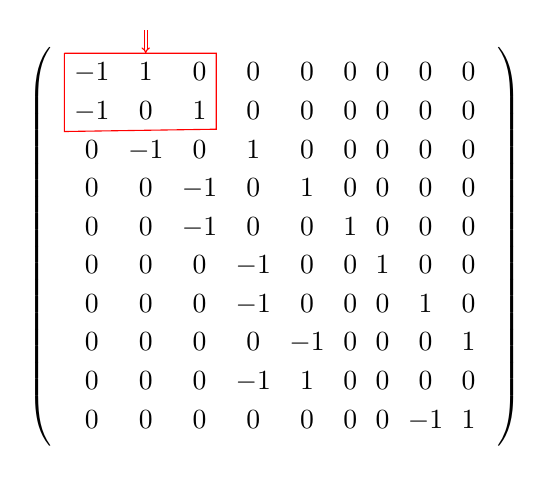
\begin{tikzpicture}
	\matrix [matrix of math nodes,left delimiter=(,right delimiter=)] (m)
	{
		-1 & 1  & 0  & 0  & 0  & 0 & 0 & 0  & 0 &  \\
		-1 & 0  & 1  & 0  & 0  & 0 & 0 & 0  & 0 &  \\
		0  & -1 & 0  & 1  & 0  & 0 & 0 & 0  & 0 &  \\
		0  & 0  & -1 & 0  & 1  & 0 & 0 & 0  & 0 &  \\
		0  & 0  & -1 & 0  & 0  & 1 & 0 & 0  & 0 &  \\
		0  & 0  & 0  & -1 & 0  & 0 & 1 & 0  & 0 &  \\
		0  & 0  & 0  & -1 & 0  & 0 & 0 & 1  & 0 &  \\
		0  & 0  & 0  & 0  & -1 & 0 & 0 & 0  & 1 &  \\
		0  & 0  & 0  & -1 & 1  & 0 & 0 & 0  & 0 &  \\
		0  & 0  & 0  & 0  & 0  & 0 & 0 & -1 & 1 &  \\
	};  
	\draw[color=red] (m-1-1.north west) -- (m-1-3.north east) -- (m-2-3.south east) -- (m-2-1.south west) -- (m-1-1.north west);
	\draw[color=red,double,implies-](m-1-2.north) -- +(0,0.3);
\end{tikzpicture}

\caption{Incidence matrix correspondig to graph in figure~\ref{fig:M1}. 
The first column corresponds to the tree root, it can be dropped. 
Green and blue submatrixes correspond to tree-edges and loop-edges, 
respectively. The tree-edge submatrix is lower triangular.}
\label{fig:M2}
\end{figure}

\newpage

\textbf{Properties of the oriented incidence matrix $D$ and other facts}

\bigskip

\underline{Dropping the root column of $D$}

\bigskip

We can rewrite the minimization problem in matrix form as follows:

$$E(x) = \sum_{(i,j) \in E} ||dx_{ij} - v_{ij}||^2 = || D x - v||^2$$

Note that as we are dealing with an integration problem, the solutions 
are equivalent \textit{modulo a translation}. The consequence of this 
fact is that we can fix the value of the tree root (ie. $x_1 = 0$). 
Thus we can drop the first column of $D$. (See 
figure~\ref{fig:M2})

\bigskip

\underline{Relation to the \textit{Laplacian} matrix and rank of $D$}

\bigskip

The directed incidence matrix has the following property:

$$L = D^t D$$

where $L$ is the \textit{Laplacian} matrix of $G$. The rank of 
$L$ is: $n-c$ (where $c$ is the number of connected components of $G$). 
In our case, as $G$ is connected, the rank of $L$ (and consequently the 
rank of $D$) is $n-1$.

\bigskip

\underline{The problem is equivalent to solve a linear system}

\bigskip

To solve the minimizatiom problem is equivalent to find where the 
gradient of $E(x)$ vanishes:
 
$$\nabla E = [\frac{\partial E}{\partial x_1}, \dots, \frac{\partial 
E}{\partial x_n}] = D^tDx-D^tv=0$$

It is equivalent to solve the linear system:

$$D^tDx = D^tv$$

As the rank of $D$ is $n-1$, the linear system may not have a solution. 
But solving the problem by iterative methods will converge to the 
closest ``possible" guess.

\bigskip

\underline{The full rank matrix $M$ based on $D$}

\bigskip

A full rank $E \times E$ matrix can be constructed based on $D$. We 
drop the first column of $D$ (as pointed before) to obtain $D'$ (a $E 
\times (V-1)$ matrix). Suppose that we rewrite $D'$ as follows:

\begin{equation}
     D'=\begin{bmatrix}
         T \\
         L
	\end{bmatrix}
 \end{equation}

Where the rows of $T$ correspond to tree edges and the rows of $L$ to 
loop-edges. We can append $E-V+1$ linearly independent columns 
spannning the orthogonal complement of $D'$:

\begin{equation}
     D'=\begin{bmatrix}
         T B\\
         L I
	\end{bmatrix}
\end{equation}

Where $I$ is the indentity matrix and the following orthogonality 
condition is satisfied: 

\begin{equation}
     0=\begin{bmatrix}
         T \\
         L
	\end{bmatrix}^t
	\begin{bmatrix}
         B\\
         I
	\end{bmatrix}
\end{equation}

This implies that

$$B = -(L)^{-t}A^t$$

The minimization we are intended to solve is equivalent to solve this 
linear system:

\newpage

TODO: Tengo que entender la matriz B del apunte de Gabriel.


Otras partes:

- Descripción del problema de Poisson y Laplace
- Mostrar ejemplo simple de que la elección del árbol generador es 
fundamental
- Problema combinatorio de elegir mejor árbol generador. Es NP? Se puede 
atacar con métodos exctos y heurísticos?
\end{document}
